\chapter{The communication model}

Shannon developed a mathematical model of the communication among parties. In particular, we will not consider the simplest one, in which the communication is one-way between two entities. In this model, one entity is the \emph{source} that sends information to the second entity, called the \emph{receiver}, through a \emph{noisy channel}.

\begin{figure}[h!]
	\centering
	\includegraphics[width=0.6\linewidth]{pictures/comm-channel.eps}
	\caption{Graphic model of a simple communication.}
\end{figure}

Source and receiver are usually separated in space and communicate (approximately) at the same time. Indeed, the roles of space and time can be swapped (i.e. a communication that evolves over time at the same place, like data storage and retrieval).

The noisy channel is both the veicle and the obstacle. One cannot transmit a signal without it being modified to some extent; moreover the communication must be quick because time is expensive. The alterations to the message are errors and therefore must be corrected. In order to do this we need to remove ``bad'' redundancy and add ``good'' redundancy. So we have a tradeoff between data integrity and fast communication.

\begin{figure}[h!]
	\centering
	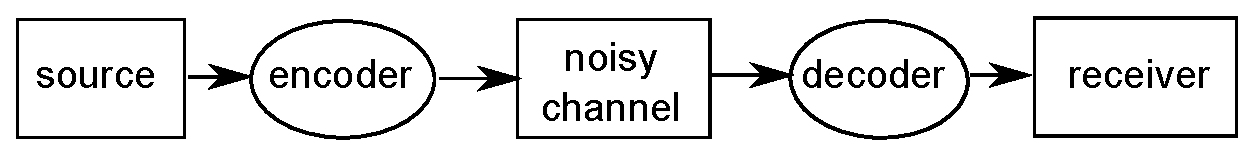
\includegraphics[width=0.9\linewidth]{pictures/comm-channel1.eps}
	\caption{The role of encoder and decoder.}
\end{figure}

The balance is found by the \emph{encoder}. This entity takes the message from the source, modify it in some way, and transmit the result over the channel. A \emph{decoder} is the entity that apply some transformation to the incoming flow of information before handling it to the receiver. The decoder can't perform the inverse of the encoder's function, because the channel applies noise to the information. We will concentrate on the noisy channel, without considering encoder and decoder's interfaces to source and receiver.

%NOTE: here he said something on asimptotic equipartition

\section{Discrete Memoryless Channel (DMC)}

For now, the channel is a black box. Let $\xset$ be the input alphabet and $\yset$ be the output alphabet for the strings that respectively enter and exit the channel. Select an input symbol $x \in \xset$; a random symbol $y \in \yset$ comes out of the channel.

We can think that there is a ``devil'' inside the black box (yes, you've read correctly, lol). The devil has dices that have $|\yset|$ faces. Whenever an input signal enters the channel, the devil launches a dice and outputs the symbol on the facet that comes up. The devil can't launch any dice; instead, there is a mapping between dices and input symbols (you can think of $x$ as the name of the dice that the devil has to use). So we can influence the devil in using some specific dice (out of the $|\xset|$ dices), but the outcome is still stochastic. The probability distribution of each dice is arbitrary. Note that the channel is usable if e have different dices; otherwise, the output is completely uncontrollable.


Let $W(y|x)$ be the probability that the dice named $x$ will fall onto its facet $y$, with the following conditions: 
\begin{itemize}
	\item 
	$W(y|x) \geq 0$,
	\item $\forall x \sum_{y \in \yset} w(y|x) = 1$.
\end{itemize}

We can think of $W$ as a matrix whose columns are indexed by $y$ and rows are indexed by $x$.

To communicate iteratively pick $x_1,x_2, \ldots, x_n \in \xset^n$ and launch a sequence of dices. There is a probability distribution for $y_1, y_2, \ldots, y_n \in Y^n$. Consider the function
\[
W^n(\str{x}, \str{y}): \xset^n \rightarrow \yset^n
\]
defined as
\[
W^n(\str{x}, \str{y}) = \prod_{i = 1}^n W(y_i | x_i)
\]

We assume that every symbol is independently modified (lack of memory of the channel). We can now define the DMC (over time instants) as
\[
\emph{DMC} = \{W^n\}_{n = 1}^\infty
\]

\section{Shannon's Noisy Channel Theorem}

The encoder takes the messages of the source and maps it to an arbitrary subset $C \subseteq \xset^n$. So we have $|C|$ many messages that flow in the channel; they can be non-binary strings, but to have an approximation of their length we can assume they are binary. Then, the length of these messages is $\log_2|C|$. We define the speed of the channel as $$\dfrac{1}{n}\log_2|C|,$$ where $n$ is the length of transmission in some unit of time. We can call this \emph{rate} of the code.

Now we are interested in the quality of transmission, that is how well data transmitted can be recovered. The decoder is a function $\varphi: \yset^n \rightarrow C$. An error event happens when $\str{x} \in \xset^n$ is transmitted and $\varphi(\str{y}) \not= \str{x}$. Define $$W^n(T|\str{x}) = \sum_{\str{y} \in T}W^n(\str{y}|\str{x}),$$

where $T \subseteq \yset$. The error probability of a string $\str{x} \in \xset^n$ is $$1 - W^n(\varphi^{-1}(\str{x})|\str{x}) = W^n(\overline{\varphi^{-1}(\str{x})}|\str{x})$$ where $$\varphi^{-1}(\str{x}) = \{\str{y}\ |\ \varphi(\str{y}) = \str{x} \}$$

Define the (maximum) error probability of the code $(C_n, \varphi_n)$ ($W^n$ is fixed) as 
\[
e_m(W^n, C_n, \varphi_n) = \max_{\str{x} \in C} W^n(\overline{\varphi^{-1}(\str{x})}, \str{x}).
\]

\begin{prop}
	$R \geq 0$ is an \emph{achievable rate} of transmission over the DMC $\{W\}$ if exists $\{(C_n, \varphi_n)\}_{n=1}^\infty$ such that:
	\begin{itemize}
		\item $\lim_{n \rightarrow \infty} \dfrac{1}{n}\log_2(|C_n|) \geq R$, and
		\item $\lim_{n \rightarrow \infty} e_m(W, C_n, \varphi_n) = 0$.
	\end{itemize}
\end{prop}

What is the highest achievable rate? $$C \subseteq \xset^n \Rightarrow \dfrac{1}{n}\log_2|C| \leq \log_2|\xset^n|$$
So the maximum achievable rate is $\log_2|\xset^n|$. Also, if $R_t \rightarrow R$ and $R_t$ is a series of values representing achievable rates, then $R$ is an achievable rate too (simple analysis, will not be demonstrated).

Shannon wondered about the highest achievable rate $C(W)$ of a given DMC $\{W\}$. He called this number \emph{capacity of the channel}. The answer came out of his intuition but it has been proved true by his students and coworkers.

Let $x \in\xset$ be a symbol chosen following a probability distribution $P|\xset$. The input symbol will be sent through the channel $W$ and the output is conditioned by $W$. Let $Y$ be the random variable (RV), $Y \in \yset$, be the output of $W$ with respect to input $X$. Then, we have a joint distribution $P, W | \xset \times \yset$. The probability that a specific input $x$ corresponds to a received symbol $y$ is
\[Pr\{X=x, Y=y\} = P(x)W(y|x).\]

Define $I(X \wedge Y)$ to be the number of bits that one can transmit over a channel in a unit of time. Intuitively, it is what $y$ retains of input $x$ (mutual information). We can maximize $I$ by controlling the probability distribution $P|\xset$ (pardon the abuse of notation): $$\max_{P|\xset}I(P, W)$$

So, what is the formula for $I$?

\[
I(X \wedge Y) = \sum_{(x, y)\in X\times Y} Pr\{X=x, Y=y\}\log_2\left(\dfrac{Pr\{X=x, Y=y\}}{Pr\{X=x\}Pr\{Y=y\}}\right) =
\]

\[
= \sum_{x \in X,  y\in Y} Pr\{X=x\}W(y|x)\log_2\left(\dfrac{Pr\{X=x\}W(y|x)}{\sum_{x\in X}Pr\{X=x\}W(y|x)}\right) = I(P, W)
\]

\begin{thm}[Shannon's Noisy Channel Theorem]\label{thm:nct}
	The highest achievable rate, given a DMC $W$, is $$C(w) = \max_{P|X}I(P, W).$$
\end{thm}

Notice that $C(W)$ is 0 if $X$ and $Y$ are independent $\Leftrightarrow$ all rows in $W$ are the same. 

\section{Binary Symmetric Channel}

A binary symmetric channel is used to transmit binary strings and the DMC has the form
\[
W = \left({\begin{array}{cc}
	1-p & p\\
	p & 1-p\\
	\end{array}}\right), \xset = \yset = \{0, 1\}
\]

It is called symmetric because $W$ is. In this context $P|\xset$ is called \emph{crossover} probability. The (hypothetical, since we proved nothing) capacity of this channel according to Theorem \ref{thm:nct} is:
\[I(X \wedge Y) = H(Y) - H(Y|X) \leq 1 -h(p)\]

This is true because:
\begin{itemize}
	\item the maximum value for $H(Y)$ is 1;
	\item the following equations hold:
	\[H(Y|X) = \sum_{x\in X}Pr\{X=x\}H(Y|X=x) = h(p),\] where 
	\[H(Y|X=x) = \sum_{y \in Y}Pr\{Y=y|X=x\}\log_2\left(\dfrac{1}{Pr\{Y=y | X=x\}} \right).\]
\end{itemize} 

Is this upper bound achievable? We must make sure that $$\exists X\ H(Y) =1$$
We can impose the uniform distribution when picking the input values, i.e. $Pr\{X = 0\} = \ifrac{1}{2}$.

We will show that $1-h(2p)$ is an achievable rate if $p < \ifrac{1}{4}$. We will to this using error correcting codes.